% A Logarithmic Cone of Prime Differences — Version 1.1
% Compile with: xelatex main.tex (twice)
\documentclass[11pt,a4paper]{article}

% ---------- Fonts ----------
\usepackage[sc]{mathpazo}
\usepackage[no-math]{fontspec}
\setmainfont{TeX Gyre Pagella}
\setsansfont{Inter}[UprightFont=*-Regular,BoldFont=*-Bold,ItalicFont=*-Italic,BoldItalicFont=*-BoldItalic,
  FontFace={sb}{n}{*-SemiBold},Scale=0.92]
\setmonofont{Latin Modern Mono}[Scale=0.95]
\newcommand{\sbseries}{\fontseries{sb}\selectfont}

% ---------- Layout ----------
\usepackage[a4paper,top=30mm,bottom=30mm,left=35mm,right=35mm,headsep=10mm]{geometry}
\usepackage{amsmath,amssymb}
\usepackage{graphicx}
\usepackage{booktabs}
\usepackage{array}
\usepackage{enumitem}
\usepackage[table]{xcolor}
\usepackage[most]{tcolorbox}
\usepackage{titlesec}
\usepackage{fancyhdr}
\usepackage[font={sf,small},labelfont={color=accent},labelsep=period,justification=raggedright,singlelinecheck=false,skip=6pt]{caption}
\usepackage{microtype}
\usepackage{xurl}
\usepackage[hidelinks]{hyperref}
\hypersetup{colorlinks=true,linkcolor=accent,citecolor=accent,urlcolor=accent}

\definecolor{accent}{HTML}{2266C4}
\definecolor{ink}{HTML}{1A1A1A}
\definecolor{muted}{HTML}{5F6670}
\definecolor{glance}{HTML}{1E7A45}
\definecolor{glancebg}{HTML}{EEF6F0}
\definecolor{claimbg}{HTML}{F1F4F9}
\definecolor{warn}{HTML}{A85A00}
\definecolor{warnbg}{HTML}{FCF3E6}

\setlength{\parindent}{0pt}
\setlength{\parskip}{0.55em}
\linespread{1.06}

% ---------- Headings ----------
\titleformat{\section}{\sffamily\bfseries\LARGE\color{ink}}{\color{accent}\thesection}{0.45em}{}
\titleformat{\subsection}{\sffamily\bfseries\large\color{ink}}{\color{accent}\thesubsection}{0.45em}{}
\titlespacing*{\section}{0pt}{1.6em}{0.7em}
\titlespacing*{\subsection}{0pt}{1.2em}{0.5em}
\newcommand{\para}[1]{\textsf{\bfseries #1}\hspace{0.45em}}

% ---------- Running heads ----------
\pagestyle{fancy}
\fancyhf{}
\renewcommand{\headrulewidth}{0pt}
\renewcommand{\sectionmark}[1]{\markboth{\thesection\quad #1}{}}
\fancyhead[L]{\sffamily\small\color{muted}\leftmark}
\fancyhead[R]{\sffamily\small\color{muted}\thepage}

% ---------- Boxes ----------
\newcommand{\notetitle}[2]{\par\noindent{\sffamily\bfseries\footnotesize\color{#1}\MakeUppercase{#2}}\par\smallskip}
\newtcolorbox{notebox}[3]{enhanced,colback=#2,colframe=#2,boxrule=0pt,arc=0pt,
  borderline west={2.5pt}{0pt}{#1},left=10pt,right=10pt,top=8pt,bottom=8pt,
  fontupper=\rmfamily\mdseries\normalsize\color{ink},before upper={\notetitle{#1}{#3}}}

\begin{document}

% ================= Title page =================
\thispagestyle{empty}
\vspace*{-4mm}
{\sffamily\small\color{muted} EXPOSITORY NOTE \quad·\quad October 2026 \quad·\quad Version 1.1\par}
\vspace{7mm}
{\sffamily\bfseries\fontsize{21}{26}\selectfont\color{ink}
A Logarithmic Cone of Prime Differences: An Expository Experiment on the Zeros of the Riemann Zeta Function\par}
\vspace{6mm}
{\sffamily\bfseries\normalsize Rodrigo Pino Osorio\par}
\vspace{1mm}
{\sffamily\small\color{muted} Independent Researcher, Viña del Mar, Chile \quad·\quad \href{mailto:paropc71@hotmail.com}{paropc71@hotmail.com}\par}
{\sffamily\small\color{muted} ORCID \href{https://orcid.org/0009-0002-1294-9136}{0009-0002-1294-9136}\par}
\vspace{5mm}
{\color{muted!40}\hrule}
\vspace{5mm}

{\small\itshape This note was written by an engineer without formal training in analytic number theory. It records an experiment and the evolution of its protocol, including the controls, the corrections and one failed test.\par}
\vspace{2mm}

\begin{notebox}{glance}{glancebg}{At a glance}
\begin{itemize}[leftmargin=1.1em,itemsep=0.35em,topsep=0pt]
\item \textbf{What was done.} The matrix of differences $p_j-p_i$ forms a smooth cone (the Prime Number Theorem). Its residual, analysed in the variable $\ln p$ for all primes up to $10^9$, shows spectral peaks at all 29 zeros of $\zeta(s)$ with $\gamma\le 100$.
\item \textbf{How strong.} Random sequences of the same density (99 Cramér and 99 Cramér-mod-30, at $X=10^8$) never reach the count of the primes ($p=0.01$, the smallest attainable with 99 sequences).
\item \textbf{What did not hold.} A pre-registered confirmation on 16 unexamined zeros met two of its three criteria and \emph{failed} the third: robustness on half-windows.
\item \textbf{What it is not.} Not new mathematics, nothing about the Riemann Hypothesis, and far less precise than established methods.
\end{itemize}
\end{notebox}

\vspace{2mm}
{\sffamily\bfseries\normalsize Abstract\par}
\vspace{1mm}
The matrix of differences $p_j-p_i$ of the primes opens like a cone, the Prime Number Theorem written geometrically. We subtract the cone and ask whether its residual carries the oscillations predicted by the explicit formula of Riemann and von Mangoldt. It does. We report the full path: negative and positive controls, two pitfalls found and corrected, and a pre-registered confirmation on 16 previously unexamined zeros that met two of its three criteria and failed the robustness test on half-windows.

\clearpage

% ================= 1 =================
\section{A picture, and a question about what it leaves out}

This note began with a picture. Plotting the differences $p_j-p_i$ between the $i$-th and $j$-th primes as a heat map (Figure~\ref{fig:cone}, left) shows a smooth surface that widens like a cone away from the diagonal. The shape is not mysterious. Summing the average gap $\ln p$ over $j-i$ consecutive primes gives
\begin{equation}\label{eq:cone}
D(i,j)=p_j-p_i=\sum_{k=i}^{j-1}\left(p_{k+1}-p_k\right)\;\approx\;(j-i)\,\ln p_i,
\end{equation}
which is the Prime Number Theorem (PNT) in integrated form. The cone is a visual restatement of a classical result.

The question that motivated the rest of the work is what remains after the cone is removed. The explicit formula of Riemann and von Mangoldt~\cite{vm} says that the distribution of primes is a smooth term plus one oscillation for each non-trivial zero $\rho=\tfrac12+i\gamma$ of $\zeta(s)$. If so, the residual of the cone should not be pure noise, and a spectral analysis should reveal those oscillations at frequencies $\gamma$.

\begin{notebox}{accent}{claimbg}{What this note does not claim}
No new result about primes or about the zeros of $\zeta(s)$, and nothing about the Riemann Hypothesis. No competition in precision: Main and collaborators recovered thousands of zeros to about twelve digits by harmonic inversion of a signal built on prime powers~\cite{main}. What we offer is an expository experiment: the residual of an object in \emph{index} space is enough to recover the zeros; the protocol is explicit and controlled; and the pitfalls, including a failed test, are reported.
\end{notebox}

% ================= 2 =================
\section{The zeros live in the logarithmic variable}

\para{The explicit formula.} For Chebyshev's function $\psi(x)=\sum_{p^k\le x}\ln p$,
\begin{equation}\label{eq:explicit}
\psi(x)=x-\sum_{\rho}\frac{x^{\rho}}{\rho}-\ln(2\pi)-\tfrac12\ln\!\left(1-x^{-2}\right),
\end{equation}
with the sum over the non-trivial zeros in symmetric order~\cite{vm}. With $\rho=\tfrac12+i\gamma$, each term behaves like $x^{1/2}e^{i\gamma\ln x}$: it is periodic in $\ln x$, not in $x$.

Berry and Keating read the explicit formula as a trace formula in which primes play the role of periodic orbits of length $\ln p$~\cite{bk}. Conrey's survey shows a Fourier transform of the PNT error term with spikes at the zeros~\cite{conrey}, and Mazur and Stein build an introductory book around this ``spectrum of the primes''~\cite{ms}.

\begin{figure}[t]
\centering
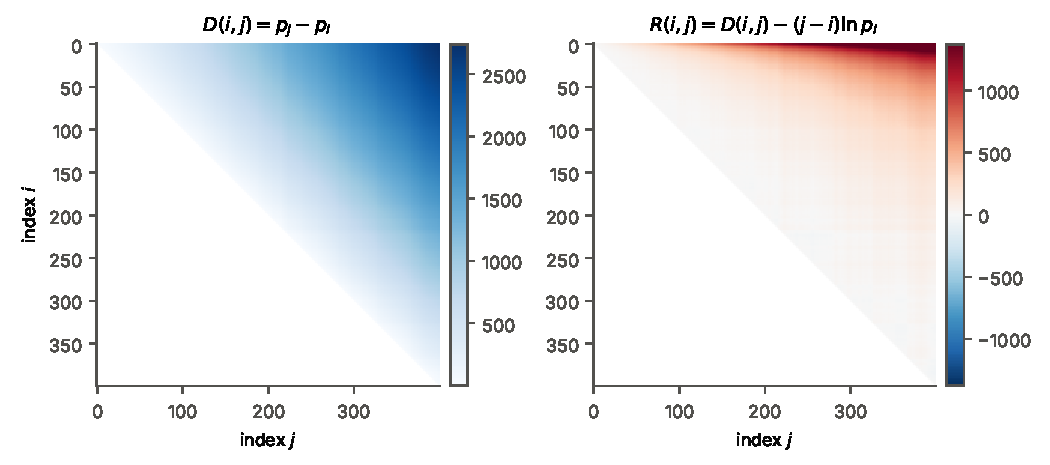
\includegraphics[width=\linewidth]{figures/fig1_cone.pdf}
\caption{The difference matrix opens like a cone; at this scale its residual is dominated by smooth curvature. Left: $D(i,j)=p_j-p_i$ for the first 400 primes. Right: the residual after subtracting $(j-i)\ln p_i$. The large-scale pattern comes from $\ln p$ varying along long spans and is removed in the analysis (Section~\ref{sec:method}). The oscillations studied here are invisible to the eye in this picture.}
\label{fig:cone}
\end{figure}

\para{Gap studies in linear variables find arithmetic, not zeros.} Spectral and correlation studies of prime gaps in linear variables found a period-three oscillation in the histogram of gap increments~\cite{kumar}, patterns in the gaps between gaps~\cite{szpiro04} and in power spectra of higher-order gaps~\cite{szpiro07}, an explanation through Hardy--Littlewood-type heuristics~\cite{ares}, and Bragg-like peaks in rational ratios in the structure factor of the primes~\cite{zmt}. None reports the zeros of $\zeta(s)$, as expected.

\para{Random models as negative controls.} Cramér's model keeps each integer $n$ independently with probability $1/\ln n$~\cite{cramer}. It reproduces the density of the primes but carries no zeros of $\zeta(s)$. Gallagher showed that, under a Hardy--Littlewood hypothesis, prime counts in short intervals are asymptotically Poisson, as that model predicts~\cite{gallagher}.

\para{This note starts from a different object.} The present experiment starts from the matrix of differences $p_j-p_i$ in index space. After the smooth cone of the PNT is removed, its residual, read in the logarithmic variable, carries spectral peaks at the zeros. No explicit use is made of the von Mangoldt function or of prime powers; the only input is the sequence of primes. Strictly, this measures $\theta(x)=\sum_{p\le x}\ln p$ rather than $\psi(x)$. Their difference, $\theta(x^{1/2})+\theta(x^{1/3})+\dots$, is dominated by the smooth term $x^{1/2}$; its oscillating part is weaker by a factor of order $x^{-1/4}$ and sits at the frequencies $\gamma_n/2$. The contribution is one of perspective, not of precision.

% ================= 3 =================
\section{From the residual of the cone to a spectrum}\label{sec:method}

All computations use the primes up to $X=10^9$ (50\,847\,534 primes), produced by a segmented sieve and checked against the known values of $\pi(x)$ for $x=10^4,\dots,10^9$. We describe the final protocol (v3). Earlier versions are discussed in Section~\ref{sec:pitfalls}.

\para{The residual.} For a span of $v$ consecutive primes,
\begin{equation}\label{eq:residual}
R_v(i)=\left(p_{i+v}-p_i\right)-v\ln p_i
\end{equation}
is the deviation of the actual span from the cone~\eqref{eq:cone}. Heuristically, the local density of primes (weighted by $\ln p$) is $1-x^{-1/2}\sum_\gamma e^{i\gamma\ln x}+\dots$, and a span is inversely proportional to the mean density over it. So $R_v$ contains a term proportional to $v\ln x\cdot x^{-1/2}\sum_\gamma\cos(\gamma\ln x+\varphi_\gamma)$, on top of smooth corrections and large gap-to-gap fluctuations.

This is a heuristic, not a derivation; the series is not absolutely convergent. Two of its features proved useful: the oscillation is periodic in $t=\ln x$, and each zero's weight does not decay like $1/|\rho|$, because the residual responds to the derivative of $\psi$.

\para{From residual to spectrum.} We use each prime $p_i\ge10^4$ with $v\ln p_i/p_i<0.05$, remove the smooth trend of $R_v$ by a least-squares cubic in $t$, weight each value by $p_i^{-1/2}$, place it at $t=\ln\!\big(\tfrac{p_i+p_{i+v}}{2}\big)$, the centre of the span, and accumulate in uniform bins of width $\Delta t=2\times10^{-4}$. The weight compensates for the number of primes per bin, which grows like $x/\ln x$: with it, each bin contributes a signal of comparable size along $t$. Then
\begin{equation}\label{eq:spectrum}
A(\gamma)=\Big|\sum_b w_b\,h_b\,e^{-i\gamma t_b}\Big|,\qquad 10\le\gamma\le100,
\end{equation}
where $w_b$ is the sum of the weighted, detrended residuals in bin $b$, $t_b$ its centre and $h_b$ a Hann taper. $A$ is computed by zero-padded FFT; we checked it against direct summation (maximum relative difference of order $10^{-6}$).

\para{Resolution.} The frequency spacing is $2\pi/(t_{\max}-t_{\min})$: about 0.55, 0.58 and 0.76 for $v=10$, 100 and 1000, because the condition $v\ln p/p<0.05$ raises $t_{\min}$ for large $v$. We call this spacing the resolution. The Hann taper doubles the width of the main lobe, so zeros closer than about two spacings are at the limit of separation.

\para{Matching peaks to zeros.} The ordinates $\gamma_n$ were computed independently with \texttt{mpmath}~\cite{mpmath}. In a range with $N$ zeros we take the $N$ highest local maxima of $A(\gamma)$, refine them by parabolic interpolation, and count a zero as \emph{matched} if a selected peak lies within half the resolution.

\para{Controls and criteria.} Negative controls: 99 Cramér sequences (odd $n$ kept with probability $2/\ln n$) and 99 that respect residues coprime to 30 (probability $\tfrac{30}{8}/\ln n$), processed identically ($v=100$, $X=10^8$); the primes are compared at the same scale. The empirical $p$-value is $(1+\#\{\text{null}\ge\text{real}\})/(N+1)$, with $N=99$ in v3, so 0.01 is the smallest attainable value ($N=20$ in v1--v2, where the floor is $1/21\approx0.048$). Positive control: the classical sum $\sum_{p^k\le X}\ln p\;p^{-k/2}\cos(\gamma k\ln p)$ through the same pipeline.

Three criteria were fixed before the first run and never changed: (a)~at least 70\% of zeros matched for every $v\in\{10,100,1000\}$, on the full range and on each half; (b)~$p<0.05$ against both random models; (c)~when $v$ changes, no matched peak moves by more than half the resolution for $v=100$.

% ================= 4 =================
\clearpage
\section{Results}

\subsection{In the linear variable the zeros do not appear}

Our first attempt transformed $R_{100}(i)$ directly along the index $i$, over $10^6$ consecutive primes between about $8\times10^3$ and $1.6\times10^7$. The power spectrum was essentially flat (log--log slope 0.04), with nothing at any $\gamma_n$. Projected onto $t=\ln p$, the same residual showed peaks close to the first zeros. This exploratory contrast agrees with the gap literature: linear variables show the arithmetic of the primes; the logarithmic variable shows the zeros.

\subsection{Two pitfalls, found and corrected}\label{sec:pitfalls}

Table~\ref{tab:versions} summarises three exploratory versions, all at $X=10^9$ for the 13 zeros in $[10,60]$ (the comparison with random models at $X=10^8$). Each change was made \emph{after} seeing the previous result.

\begin{table}[h]
\caption{Each correction improved the exploratory protocol; v3 meets all three criteria on $\gamma\in[10,60]$. (a)~worst case over all $v$ and windows; (b)~$p$ and $z$ against Cramér / Cramér-mod-30 (20 sequences per model in v1--v2, 99 in v3); (c)~drift, limit in brackets; $\bar\Delta$ mean peak error for $v=100$, number of negative errors (of 13) in brackets.}
\label{tab:versions}
\centering\sffamily\small
\begin{tabular}{@{}l>{\raggedright\arraybackslash}p{2.6cm}rrrrr@{}}
\toprule
Ver. & Change & (a) & (b) $p$ & $z$ & (c) drift & $\bar\Delta$ (neg.)\\
\midrule
v1 & --- & 46\,\% & 0.048 & 7.1 / 9.0 & 0.289 (0.273) & $-0.029$ (13)\\[2pt]
v2 & filter $v\ln p/p<0.05$ & 77\,\% & 0.048 & 6.1 / 8.9 & 0.064 (0.290) & $-0.019$ (13)\\[2pt]
\textbf{v3} & \textbf{span centre, 99 nulls} & \textbf{77\,\%} & \textbf{0.010} & \textbf{7.2 / 7.5} & \textbf{0.260 (0.291)} & $\boldsymbol{+0.002}$ \textbf{(3)}\\
\bottomrule
\end{tabular}
\end{table}

\para{Pitfall 1: long spans at small primes act as a low-pass filter.} In v1, $v=1000$ on the lower half matched only 6 of 13 zeros. A span of $v$ primes covers $\Delta t\approx v\ln p/p$ in $t$, and averaging over it filters with response $|\mathrm{sinc}(\gamma\Delta t/2)|$, where $\mathrm{sinc}(x)=\sin x/x$. Near $p=10^4$ with $v=1000$, $\Delta t\approx0.9$, which suppresses higher $\gamma$; and the weight $p^{-1/2}$ makes that region count. Using only primes with $v\ln p/p<0.05$ (v2) raised the worst case to 77\% and cut the drift between values of $v$ from 0.289 to 0.064.

\para{Pitfall 2: labelling a span by its left endpoint shifts every peak.} In v1 and v2, all 13 peaks fell slightly below their zeros (sign test $p=2.4\times10^{-4}$ in v2). Spectral leakage was ruled out first: a synthetic signal with 150 zeros and no primes gave a mean shift of $+0.001$ with mixed signs.

The cause was simpler. $R_v(i)$ measures the span $[p_i,p_{i+v}]$, but v1--v2 placed it at its left end, $t=\ln p_i$. That $t$-dependent offset compresses the axis and shifts each peak down in proportion to $\gamma$. Placing spans at their centre (v3) took the mean error for $v=100$ from $-0.019$ to $+0.002$; the largest error over 13 zeros became 0.017 (Figure~\ref{fig:bias}).

\begin{figure}[t]
\centering
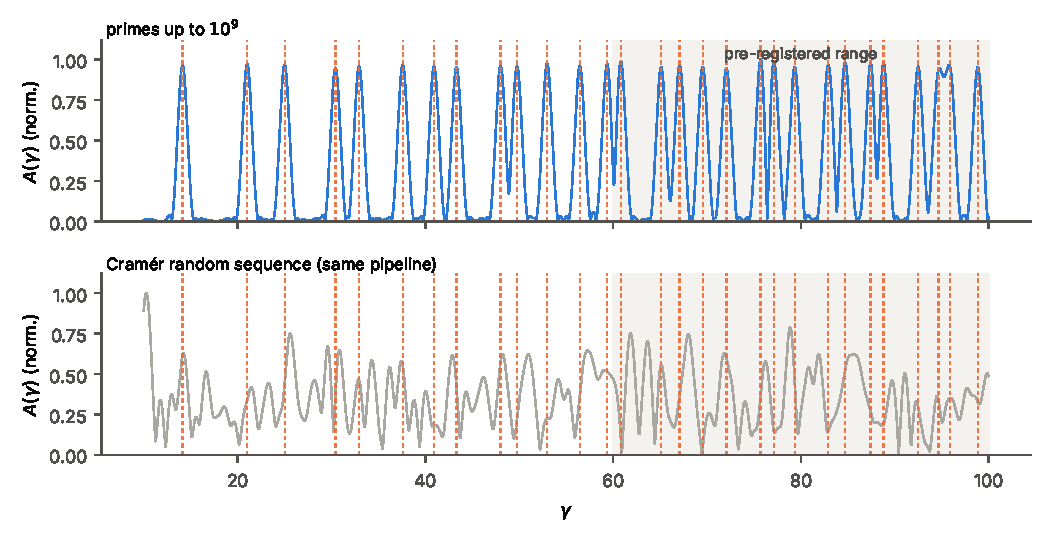
\includegraphics[width=\linewidth]{figures/fig2_spectrum.pdf}
\caption{Peaks of the residual coincide with all 29 zeros up to $\gamma=100$; a random sequence shows no such pattern. Top: $A(\gamma)$ for $v=100$, primes up to $10^9$, span-centre convention. Dashed lines: zeros of $\zeta(s)$; shaded: the pre-registered range. Bottom: one Cramér sequence through the same pipeline ($X=10^8$). Each panel normalised to its own maximum.}
\label{fig:spectrum}
\end{figure}

\begin{figure}[t]
\centering
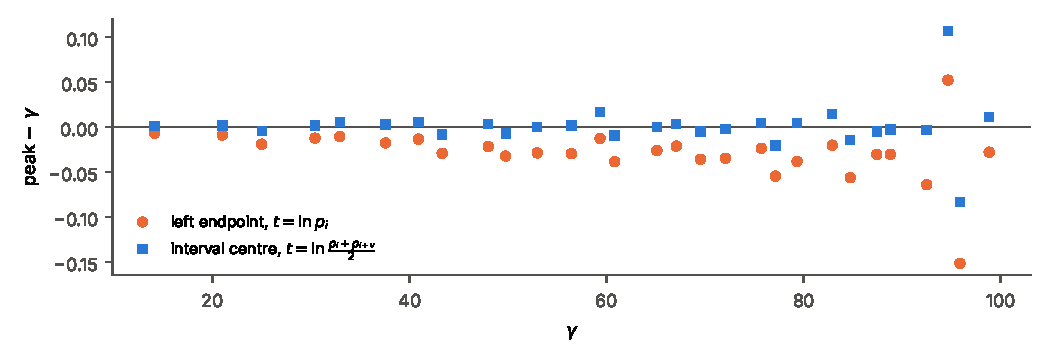
\includegraphics[width=\linewidth]{figures/fig3_bias.pdf}
\caption{Labelling each span by its centre removes the downward bias of the peaks. $v=100$, $X=10^9$, full window. Left endpoint (circles): 28 of 29 errors negative, mean $-0.029$. Centre (squares): 13 of 29 negative, mean $+0.001$. The two largest errors in both conventions sit at the close pair $\gamma\approx94.65,\ 95.87$, separated by 1.22, about two resolution spacings: the limit of separation with the Hann taper.}
\label{fig:bias}
\end{figure}

\subsection{Pre-registered confirmation: two criteria met, one failed}

To test v3 on data that played no role in its design, we froze the code and changed only the range of $\gamma$ to $[60,100]$: 16 zeros never examined before. Hypotheses, decision rule (confirm only if (a), (b) and (c) all pass) and expected risks were recorded beforehand in a document with a registered SHA-256 digest.\footnote{SHA-256 of the pre-registration document, recorded by the author on 2026-10-12, 08:22:23 UTC, before the run; the document and its digest are in the repository (folder \texttt{preregistration}):\\ \texttt{\footnotesize 883963ad640caec1fd97a9d63c6354cc1686e7ec73b5e3545ec302a7583155c1}.}

\begin{table}[h]
\caption{On new zeros the full range recovers all 16, but half-windows fall below the 70\,\% threshold. Pre-registered confirmation, $\gamma\in[60,100]$, code of v3 frozen; $X=10^9$ for (a) and (c), $X=10^8$ for (b). Zeros matched (of 16).}
\label{tab:prereg}
\centering\sffamily\small
\begin{tabular}{@{}lrrr@{}}
\toprule
 & Full range & Lower half & Upper half\\
\midrule
$v=10$ & \textbf{16} & 13 & 10\\
$v=100$ & \textbf{16} & 9 & 10\\
$v=1000$ & \textbf{16} & 6 & 11\\
\bottomrule
\end{tabular}

\vspace{4mm}
\begin{tabular}{@{}l>{\raggedright\arraybackslash}p{5.4cm}l@{}}
\toprule
Test & Result & Verdict\\
\midrule
(a) worst case & 38\,\% (threshold 70\,\%) & \textbf{not met}\\
(b) random models & primes 16; nulls mean 5.1 / 4.9, max 10 / 8; $p=0.01$, $z=6.4$ / $6.6$ & met\\
(c) drift & 0.234 (limit 0.291) & met\\
Sign bias (secondary) & span centre 10/16 negative, $p=0.45$ & met\\
Positive control & 16 / 16 & ---\\
\bottomrule
\end{tabular}
\end{table}

\begin{notebox}{warn}{warnbg}{Pre-registered verdict: not confirmed}
Criterion (a) failed, so by the rule fixed in advance the confirmation did not pass. On the new data, detection on the full range, separation from the random models, stability across $v$ and absence of bias all held; robustness on half-windows did not.
\end{notebox}

Halving the range doubles the spacing to 1.09--1.52; with the Hann main lobe, peaks closer than about twice the spacing merge, and several zeros in $[60,100]$ are only 1.22--1.38 apart. For large $v$, the residual low-pass effect also weakens the lower half. Both causes were listed in the pre-registration. That the failure occurred where anticipated is consistent with them, but it does not turn it into a success.

One expectation in our pre-registration was wrong: we expected weaker peaks at higher $\gamma$ because terms of the explicit formula carry $1/|\rho|$. Figure~\ref{fig:spectrum} shows comparable heights throughout. This agrees with the heuristic of Section~\ref{sec:method}: the residual responds to the derivative of $\psi$, where that factor cancels.

\begin{figure}[t]
\centering
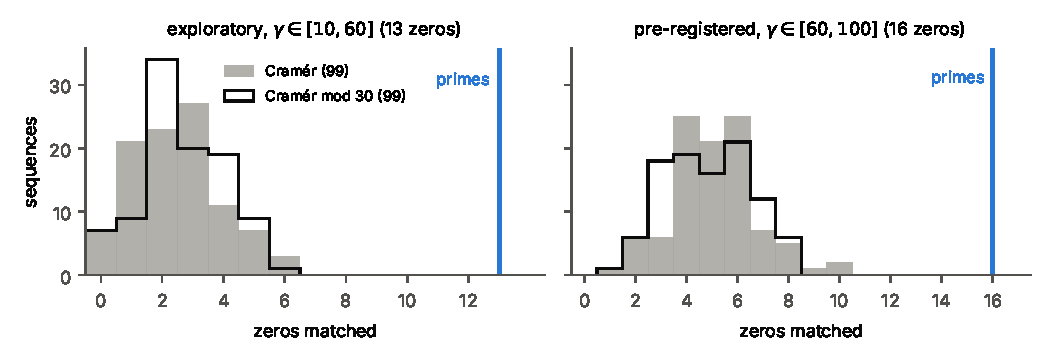
\includegraphics[width=\linewidth]{figures/fig4_nulls.pdf}
\caption{No random sequence reaches the count of the primes. Zeros matched by 99 Cramér and 99 Cramér-mod-30 sequences (histograms) and by the primes (vertical line), $v=100$, $X=10^8$. Left: exploratory range. Right: pre-registered range.}
\label{fig:nulls}
\end{figure}

\subsection{Re-runs in a separate environment reproduce the results}\label{sec:rerun}

The notebooks are deterministic with fixed seeds. The author re-ran v2 and v3 on Google Colab. For v2, every printed result coincided except running time and memory, including the match counts of all 40 null sequences.

For v3, all decisions and counts coincided; floating-point values in the result files differed by at most $5\times10^{-13}$ (relative), with a different \texttt{numpy} version (2.1.3 versus 2.5.3). The pre-registered confirmation was run once and has not yet been reproduced independently. A full run takes about 18 minutes on two virtual CPUs and peaks at about 1.3\,GB of memory.

% ================= 5 =================
\section{What this shows, and what it does not}

\para{What it shows.} Once the smooth cone of the PNT is removed from the matrix of prime differences, what remains is not featureless. Read in $\ln p$, it shows peaks at the zeros of $\zeta(s)$, here all 29 with $\gamma\le100$, at a level random sequences of the same density do not reach. That is what the explicit formula predicts, seen from an unusual angle: an object in index space, built only from differences between primes.

\begin{notebox}{warn}{warnbg}{Limitations}
\begin{itemize}[leftmargin=1.1em,itemsep=0.35em,topsep=0pt]
\item Nothing new about the zeros; precision ($\approx10^{-2}$) is modest next to established methods~\cite{main}.
\item Amendments v2 and v3 were designed after seeing data; the only test on fresh data confirmed detection on the full range but not robustness on half-windows.
\item A single scale ($X=10^9$), simple random models, and thresholds (70\,\%, half a resolution) that are reasonable conventions rather than derived values.
\item The span filter limits but does not remove the low-pass effect: at the threshold $v\ln p/p=0.05$, the response at $\gamma=100$ is $|\mathrm{sinc}(2.5)|\approx0.24$.
\end{itemize}
\end{notebox}

\para{Lessons that may be useful to others.} Three practical points emerged that we have not seen stated together. Use the logarithmic variable: linear analyses of gaps show the arithmetic of the primes, not the zeros. Avoid spans that are long relative to $p$: a span filters with width $v\ln p/p$ in $t$. Label each span by its centre: an endpoint produces a small, systematic shift that can be mistaken for a property of the primes.

% ================= 6 =================
\section{A classical fact, seen from an unusual angle}

A picture of prime differences led to a question, and the question led to a small experiment with a clear answer. The residual of the logarithmic cone carries the spectral signature of the Riemann zeros, as the explicit formula says it should. We have tried to tell the story as it happened: with its controls, its corrections, the one test that did not pass, and no claims beyond what the data support. If the note has a value, we hope it lies there, as a reproducible and honest way of seeing a classical fact for oneself.

\vspace{3mm}
{\color{muted!40}\hrule}
\vspace{2mm}
{\sffamily\small
\textbf{Data and code availability.} All notebooks (v1--v3 and the pre-registered confirmation), the JSON result files containing every null-sequence count, and the pre-registration document with its SHA-256 digest are available at \url{https://github.com/rodpino71-expert/logarithmic-cone-zeta}, archived on Zenodo with each release. The notebooks are deterministic with fixed seeds. Requirements: \texttt{numpy}, \texttt{matplotlib}, \texttt{mpmath}.

\medskip
\textbf{License.} Text and figures: CC BY 4.0. Code: MIT.

\medskip
\textbf{Use of AI assistance.} The author built the initial visualizations that motivated this work, posed the research questions and set the direction of the analysis code, approving every change to the protocol. An AI assistant (Claude, by Anthropic) refined and extended that code under the author's instructions, ran the computations, performed the literature search and drafted this text under the author's direction. The author independently re-ran the main notebooks on Google Colab (Section~\ref{sec:rerun}) and is responsible for all interpretations.\par}

% ================= References =================
\clearpage
\renewcommand{\refname}{References}
\titleformat{\section}{\sffamily\bfseries\LARGE\color{ink}}{}{0pt}{}
\begin{thebibliography}{99}\small\markboth{References}{}
\bibitem{ares} S.~Ares and M.~Castro, Hidden structure in the randomness of the prime number sequence?, \emph{Physica A} \textbf{360} (2006) 285--296. arXiv:cond-mat/0310148.
\bibitem{bk} M.~V.~Berry and J.~P.~Keating, The Riemann zeros and eigenvalue asymptotics, \emph{SIAM Review} \textbf{41} (1999) 236--266.
\bibitem{conrey} J.~B.~Conrey, The Riemann Hypothesis, \emph{Notices Amer. Math. Soc.} \textbf{50} (2003) 341--353.
\bibitem{cramer} H.~Cramér, On the order of magnitude of the difference between consecutive prime numbers, \emph{Acta Arith.} \textbf{2} (1936) 23--46.
\bibitem{gallagher} P.~X.~Gallagher, On the distribution of primes in short intervals, \emph{Mathematika} \textbf{23} (1976) 4--9.
\bibitem{kumar} P.~Kumar, P.~Ch.~Ivanov and H.~E.~Stanley, Information entropy and correlations in prime numbers, arXiv:cond-mat/0303110 (2003).
\bibitem{main} J.~Main, V.~A.~Mandelshtam, G.~Wunner and H.~S.~Taylor, Harmonic inversion as a general method for periodic orbit quantization, \emph{Nonlinearity} \textbf{11} (1998), doi:10.1088/0951-7715/11/4/014. arXiv:chao-dyn/9709009.
\bibitem{ms} B.~Mazur and W.~Stein, \emph{Prime Numbers and the Riemann Hypothesis}, Cambridge University Press, 2016.
\bibitem{mpmath} The mpmath development team, \emph{mpmath: a Python library for arbitrary-precision floating-point arithmetic}, \url{https://mpmath.org}.
\bibitem{szpiro04} G.~G.~Szpiro, The gaps between the gaps: some patterns in the prime number sequence, \emph{Physica A} \textbf{341} (2004) 607--617.
\bibitem{szpiro07} G.~G.~Szpiro, Peaks and gaps: spectral analysis of the intervals between prime numbers, \emph{Physica A} \textbf{384} (2007) 291--296.
\bibitem{vm} H.~von Mangoldt, Zu Riemanns Abhandlung ``Über die Anzahl der Primzahlen unter einer gegebenen Grösse'', \emph{J. Reine Angew. Math.} \textbf{114} (1895) 255--305.
\bibitem{zmt} G.~Zhang, F.~Martelli and S.~Torquato, The structure factor of primes, arXiv:1801.01541 (2018).
\end{thebibliography}

\end{document}
